\chapter{Image Manipulation (2D)}

\section{Multiplanar Reconstruction}

When images are imported, InVesalius automatically shows its multiplanar reconstruction in the Axial, Sagittal and Coronal orientations, as well as a window for 3D manipulation, as seen in Figure~\ref{fig:mpr}.

\begin{figure}[!htb]
\centering
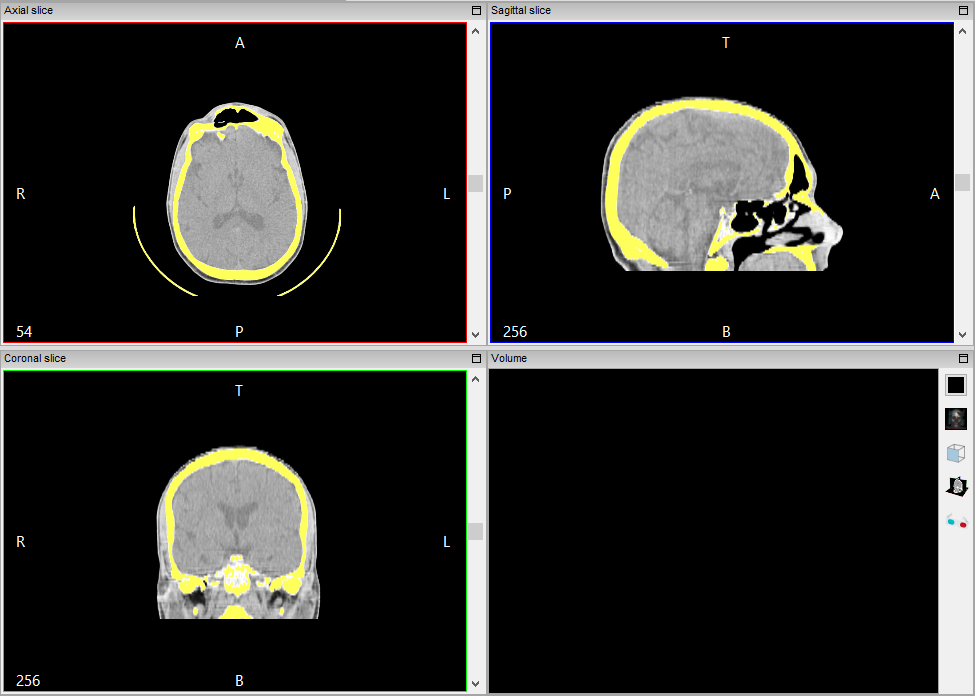
\includegraphics[scale=0.40]{multiplanar_mask_window_en.png}
\caption{Multiplanar Reconstruction}
\label{fig:mpr}
\end{figure}

\newpage

In addition to creating a multiplanar reconstruction, InVesalius segments an image, highlighting for example soft tissue bones. The highlight is represented by the application of colors on a segmented structure so that the colors form a mask over an image highlighting the structure (Figure~\ref{fig:mpr}).This is discussed in more detail in the following chapters.

To hide the mask, use the data manager, located in the lower left corner of the screen. Select the \textbf{Masks} tab and click once using the \textbf{left} mouse button over the eye icon next to \textbf{"Mask 1"}, as shown in Figure~\ref{fig:ger_masc}.

\begin{figure}[!htb]
\centering
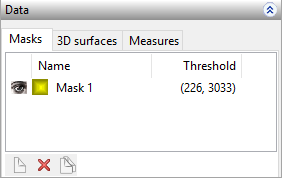
\includegraphics[scale=0.8]{data_mask_en.png}
\caption{Mask manager}
\label{fig:ger_masc}
\end{figure}

The eye icon disappears, and the colors of the segmentation mask are hidden (Figure~\ref{fig:mpr_sem_mask}).

\begin{figure}[!htb]
\centering
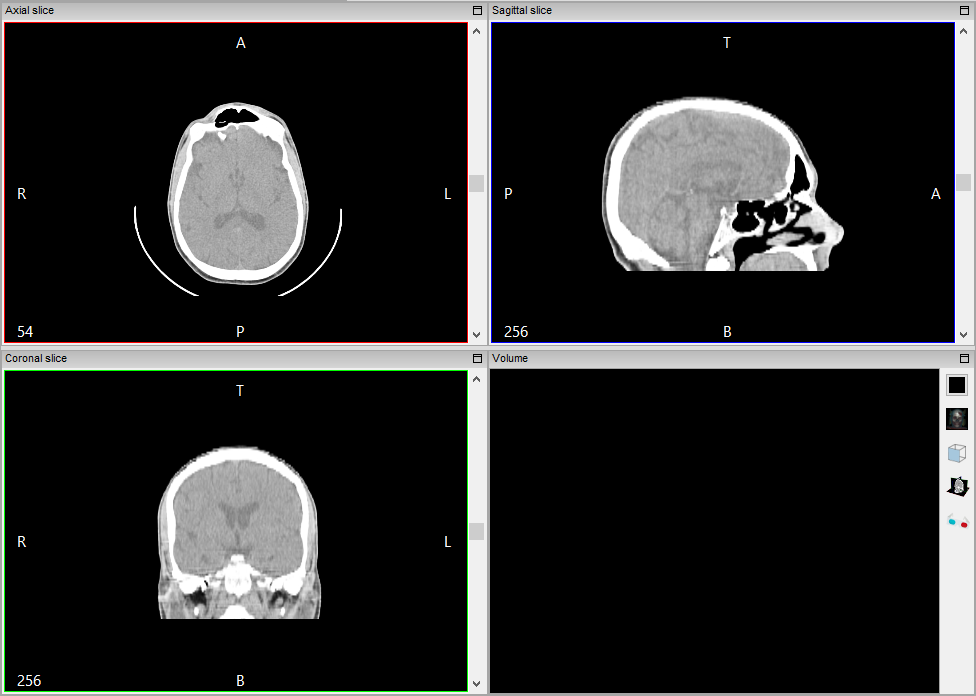
\includegraphics[scale=0.30]{multiplanar_window_en.png}
\caption{Multiplanar reconstruction without segmentation mask}
\label{fig:mpr_sem_mask}
\end{figure}

\subsection{Axial orientation}

The axial orientation consists of cuts made transversally to the region of interest, i.e. parallel cuts to the axial plane of the human body.
In Figure~\ref{fig:axial_corte}, an axial image of the skull region is displayed.

\begin{figure}[!htb]
\centering
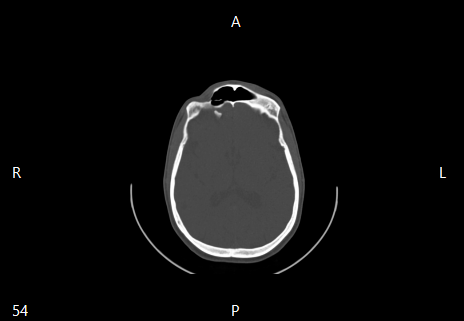
\includegraphics[scale=0.30]{axial_en.png}
\caption{Axial slice}
\label{fig:axial_corte}
\end{figure}

\subsection{Sagittal orientation}

The sagittal orientation consists of cuts made laterally in relation to the region of interest, i.e. parallel cuts to the sagittal plane of the human body, which divides it into the left and right portions.
In Figure~\ref{fig:sagital_slice}, a sagittal skull image is displayed.

\begin{figure}[!htb]
\centering
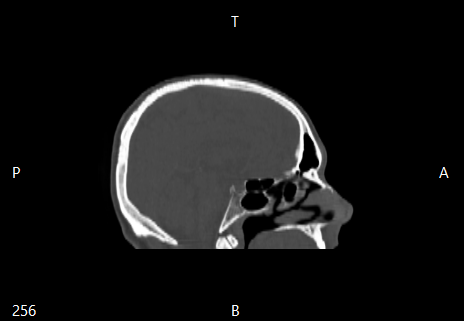
\includegraphics[scale=0.30]{sagital_en.png}
\caption{Sagittal slice}
\label{fig:sagital_slice}
\end{figure}

\newpage

\subsection{Coronal orientation}

The coronal orientation is composed of cuts parallel to the coronal plane, which divides the human body into ventral and dorsal halves.
In Figure~\ref{fig:coronal_slice} is displayed a skull image in coronal orientation.

\begin{figure}[!htb]
\centering
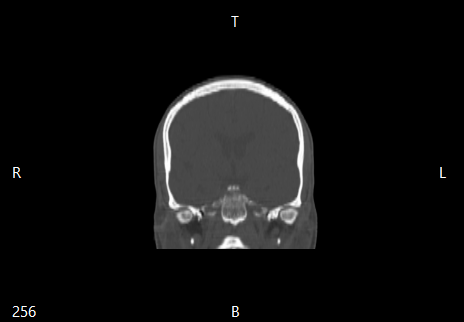
\includegraphics[scale=0.30]{coronal_en.png}
\caption{Coronal slice}
\label{fig:coronal_slice}
\end{figure}


\section{Correspondence between the axial, sagittal and coronal orientations}
\label{sec:corresp_all_orient}

To find out the common point of intersection of the images in differents orientations, simply activate the "Slices cross intersection" feature with the shortcut icon located on the toolbar. See Figure~\ref{fig:cross_icon}.

\begin{figure}[!htb]
\centering

\includegraphics[scale=1]{cross.png}
\caption{Shortcut to show common point between different orientations}
\label{fig:cross_icon}
\end{figure}

When the feature is activated, two cross-sections that intersect perpendicularly are displayed on each image (Figure~\ref{fig:cross_all}). The intersection point of each pair of segments represents the common point between differents orientations.

\newpage

To modify the point, hold down the \textbf{left} mouse button and \textbf{drag}. Automatically, the corresponding points will be updated in each image.

\begin{figure}[!htb]
\centering
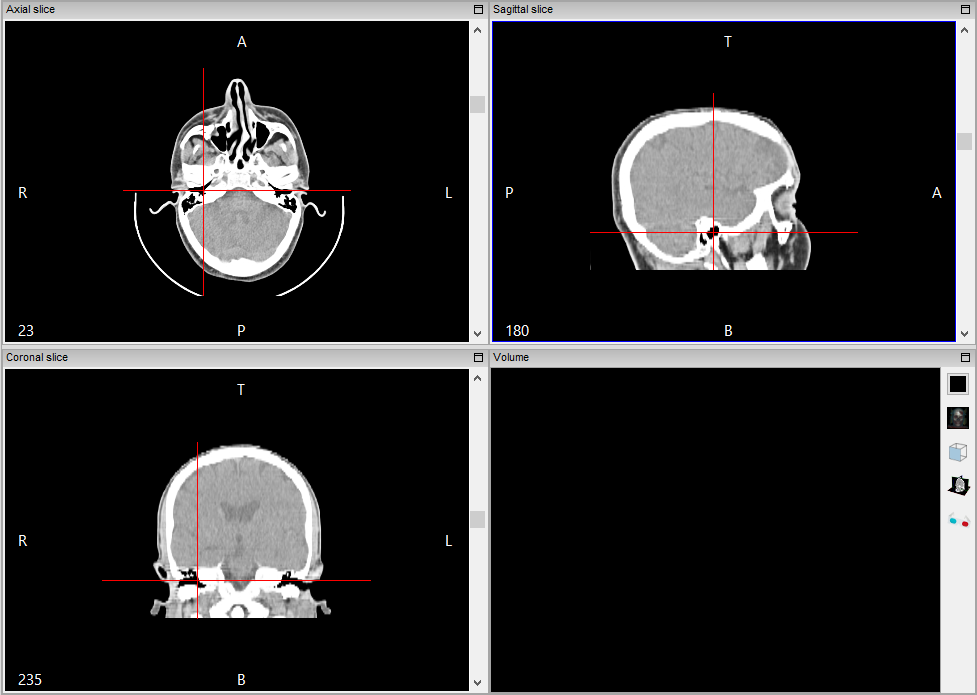
\includegraphics[scale=0.4]{multiplanar_window_cross_en.png}
\caption{Common point between differents orientations}
\label{fig:cross_all}
\end{figure}

To deactivate the feature, simply click on the shortcut again (Figure~\ref{fig:cross_icon}). This feature can be used in conjunction with the slice editor (which will be discussed later).

\section{Interpolation}

By default the 2D images visualization are interpolated (Figure~\ref{fig:interp}).a). To deactivate this feature, select the \textbf{View} menu and select \textbf{Interpolated slices} (Figure~\ref{fig:menu_interpoleted_image_pt}). It will then be possible to visualize each pixel individually as shown in Figure~\ref{fig:interp}.b.

\textbf{This interpolation is for visualization purposes only, and does not directly influence segmentation or 3D surface generation.}

\begin{figure}[!htb]
\centering
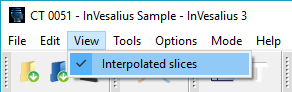
\includegraphics[scale=0.7]{menu_interpoleted_image_en.png}
\caption{Menu to disable and enable interpolation}
\label{fig:menu_interpoleted_image_pt}
\end{figure}


\begin{figure}[!htb]
  \centering
  \subfloat[Interpolated]{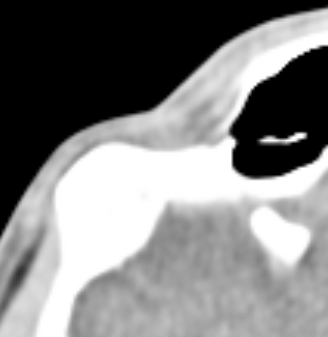
\includegraphics[width=0.4\textwidth]{axial_interpoleted.png}}  \qquad
  \subfloat[Non-interpolated]{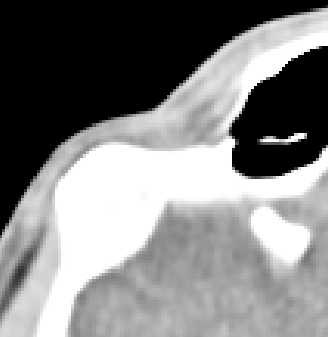
\includegraphics[width=0.4\textwidth]{axial_not_interpoleted.png}}
  \hfill
  \caption{Interpolated and non-interpolated image visualization.}
  \label{fig:interp}
\end{figure}

\section{Move}

To move an image on the screen, use the Move shortcut icon on the toolbar (Figure~\ref{fig:move_icon}). Click on the icon to activate, then with the \textbf{left} mouse button on the image, \text{drag} it to the desired direction. Figure~\ref{fig:move_img} shows a displaced (moved) image.

\begin{figure}[!htb]
\centering

\includegraphics[scale=0.25]{tool_translate_original.png}
\caption{Shortcut to move images}
\label{fig:move_icon}
\end{figure}

\begin{figure}[!htb]
\centering
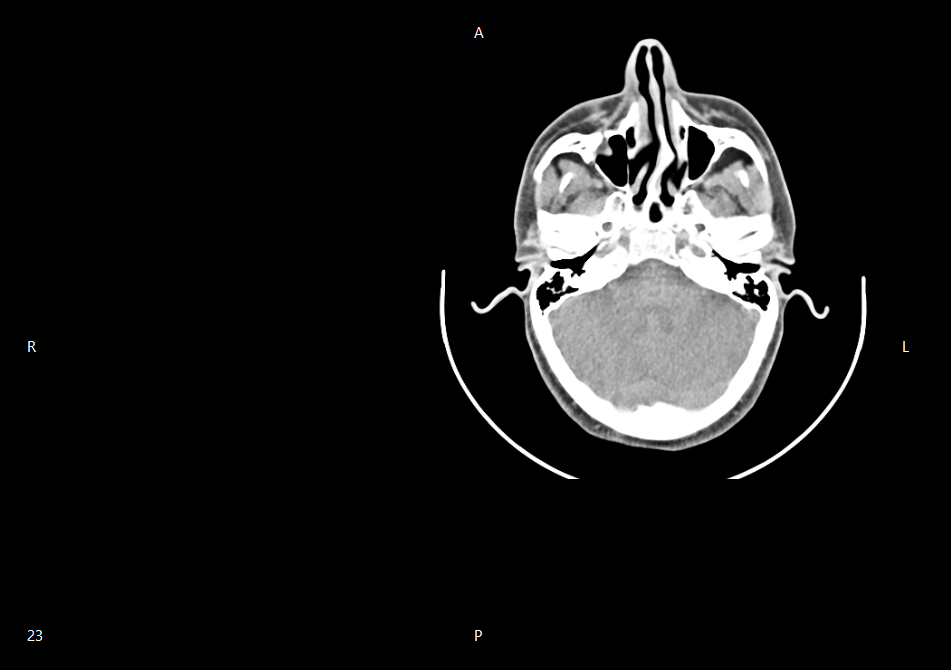
\includegraphics[scale=0.20]{axial_pan_en.png}
\caption{Displaced image}
\label{fig:move_img}
\end{figure}

\section{Rotate}

Images can be rotated by using the Rorate shortcut on the toolbar (Figure~\ref{fig:rot_icon}). To rotate an image, click on the icon and then with the \textbf{left} mouse button \textbf{drag} clockwise or anticlockwise as required.

\begin{figure}[!htb]
\centering

\includegraphics[scale=0.20]{tool_rotate_original.png}
\caption{Shortcut to rotate images}
\label{fig:rot_icon}
\end{figure}

\begin{figure}[!htb]
\centering
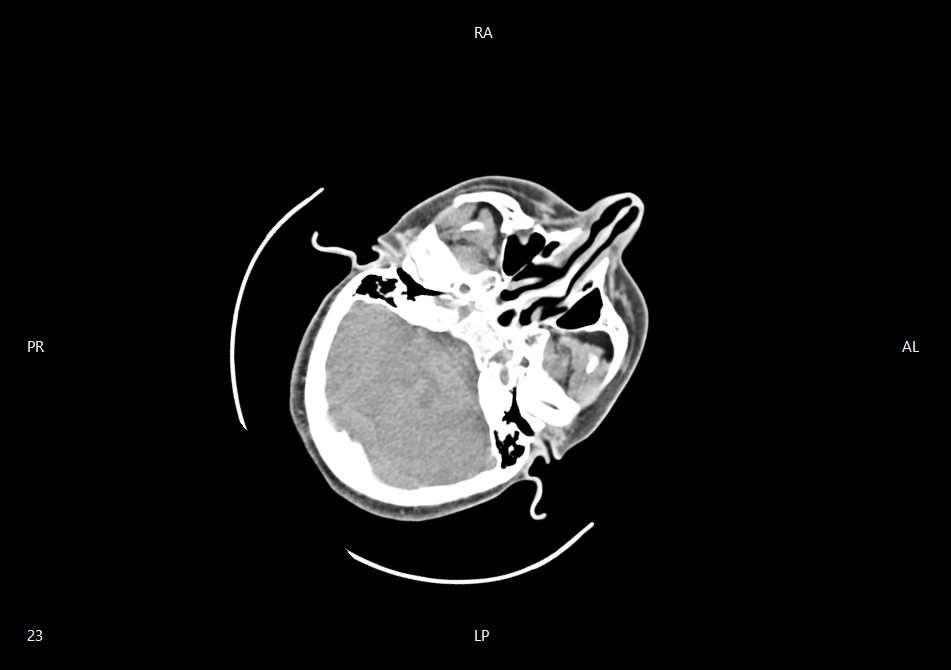
\includegraphics[scale=0.20]{axial_rotate_en.png}
\caption{Rotated image}
\label{fig:rotate_all}
\end{figure}


\section{Zoom}

In InVesalius, there are different ways to enlarge an image. You can maximize the desired orientation window, apply zoom directly to the image, or select the region of the image to enlarge. Each of these methods are detailed below.

\subsection{Maximizing orientation windows}

The main InVesalius window is divided into 4 sub-windows: axial, sagittal, coronal and 3D. Each of these can be maximized to occupy the entire area of the main window. To do this, simply \textbf{left} mouse click on the subwindow icon located in the \textbf{upper right corner} (Figure~\ref{fig:maximize_window}). To restore a maximized window to its previous size, simply click the icon again.

\begin{figure}[!htb]
\centering
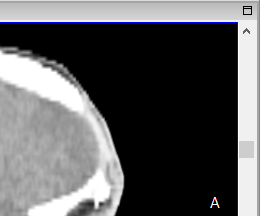
\includegraphics[scale=0.6]{maximize_sagital_mpr.png}
\caption{Detail of a sub-window (Note the maximize icon in the upper right corner)}
\label{fig:maximize_window}
\end{figure}

\subsection{Enlarging or shrinking an image}

To enlarge or shrink an image, click on the zoom shortcut icon in the toolbar (Figure~\ref{fig:zoom_icon}). Hold down the \textbf{left} mouse button on the image and \textbf{drag} the mouse \textbf{up} to enlarge or \textbf{down} to shrink.

\begin{figure}[!htb]
\centering

\includegraphics[scale=0.25]{tool_zoom_original.png}
\caption{Zoom shortcut}
\label{fig:zoom_icon}
\end{figure}

\subsection{Enlarging an image area}

To enlarging a certain image area, click on the "Zoom based on selection" icon in the toolbar (Figure~\ref{fig:zoom_icon_loc}). Position the mouse pointer at the origin point of the selection, click and hold the \textbf{left} mouse button and \textbf{drag} it to the end selection point to form a rectangle (Figure~\ref{fig:zoom_select}). Once the left mouse button is released, the zoom operation will be applied to the selected region (Figure~\ref{fig:zoom_applied}).

\begin{figure}[!htb]
\centering

\includegraphics[scale=0.25]{tool_zoom_select_original.png}
\caption{Zoom based on selection shortcut}
\label{fig:zoom_icon_loc}
\end{figure}

\begin{figure}[!htb]
\centering
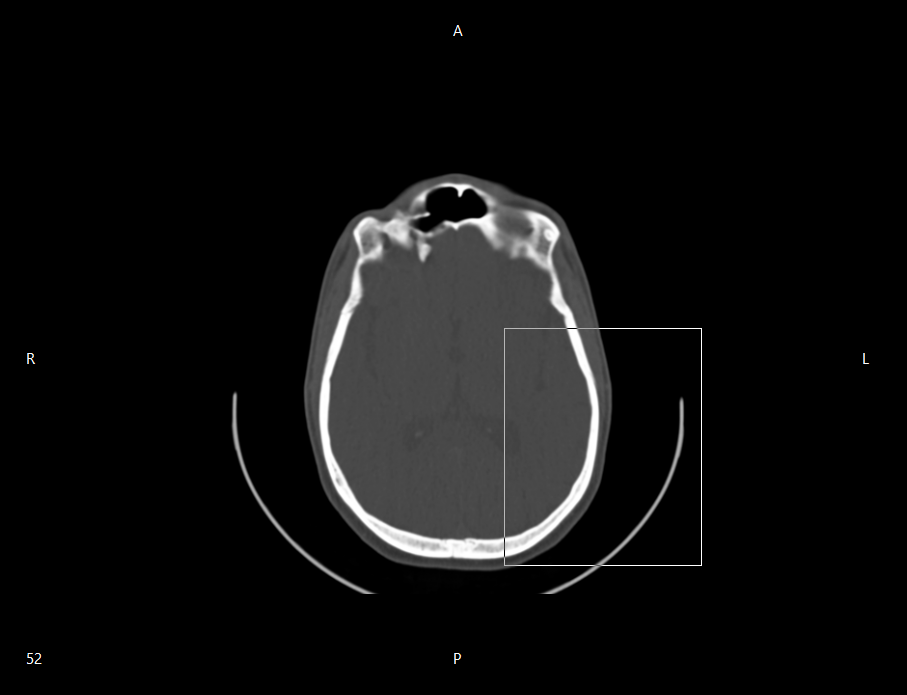
\includegraphics[scale=0.25]{tool_zoom_select_image_en.png}
\caption{Area selected for zoom}
\label{fig:zoom_select}
\end{figure}

\begin{figure}[!htb]
\centering
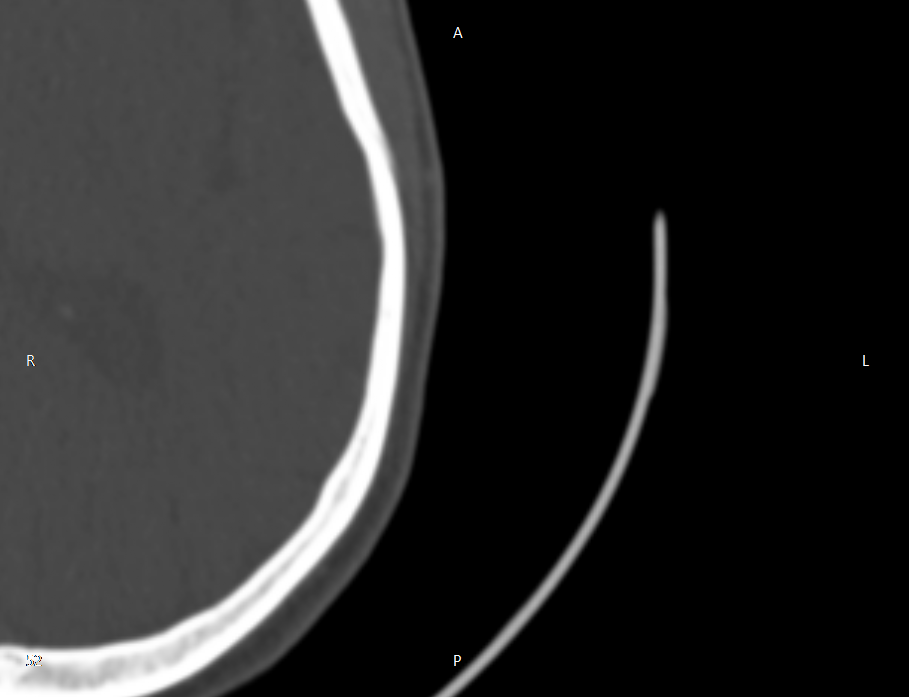
\includegraphics[scale=0.25]{tool_image_with_zoom_en.png}
\caption{Enlarged Image}
\label{fig:zoom_applied}
\end{figure}


\section{Brightness and contrast (Windows)}
\label{sec:ww_wl}

To improve image visualization, the \textit{window width} and \textit{window level} features can be used; these are more commonly known as \textit{brightness and contrast} or \textit{window} (for radiologists). With this feature, it is possible to set the range of the gray scale (\textit{window level}) and the width of the scale (\textit{window width}) to be used to display the images.

The feature can be activated by the "Brightness and Contrast" shortcut icon in the toolbar. See Figure~\ref{fig:window_level_shortcut}.

\begin{figure}[!htb]
\centering

\includegraphics[scale=0.70]{tool_contrast_original.png}
\caption{Brightness and contrast shortcut}
\label{fig:window_level_shortcut}
\end{figure}

To increase the brightness, hold down the \textbf{left} mouse button and \textbf{drag} horizontally to the right. To decrease the brightness, simply drag the mouse to the left. The contrast can be changed by dragging the mouse (with the \textbf{left} button pressed) vertically: up to increase, or down to decrease contrast.

To deactivate the feature, click again on the shortcut icon (Figure~\ref{fig:window_level_shortcut}).

Preset brightness and contrast patterns may be used with InVesalius. Table~\ref{tab:window_level} lists some tissue types with their respective brightness and contrast values. To use the presets, position the mouse cursor over an image and \textbf{right-click} to open a context menu, then select \textbf{Window width and level}, and click on the preset option according to the tissue type, as shown in Figure~\ref{fig:window_level}.

\begin{figure}[!htb]
\centering
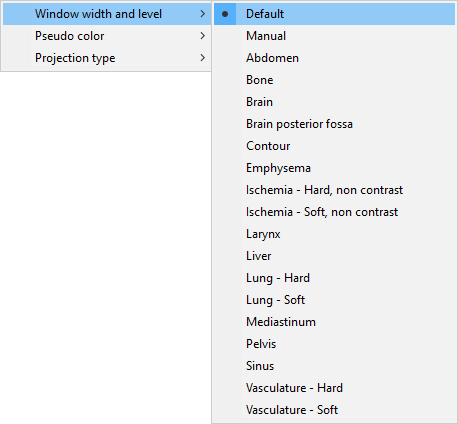
\includegraphics[scale=0.40]{menu_window_and_level_en.png}
\caption{Context menu for brightness and contrast selection}
\label{fig:window_level}
\end{figure}

\begin{table}[!h]
\centering
\caption{Brightness and contrast values for some tissues}
\begin{tabular}{lcc}\\
\hline % este comando coloca uma linha na tabela
Tissue & Brightness & Contrast\\
\hline
\hline
Default & Exam & Exam\\
Manual & Changed & Changed\\
Abdomen & 350 & 50\\
Bone & 2000 & 300\\
Brain & 80 & 40\\
Brain posterior fossa & 120 & 40\\
Contour & 255 & 127\\
Emphysema & 500 & -850\\
Ischemia - Hard, non contrast & 15 & 32\\
Ischemia - Soft, non contrast & 80 & 20\\
Larynx & 180 & 80\\
Liver & 2000 & -500\\
Lung Hard & 1000 & -600\\
Lung Soft & 1600 & -600\\
Mediastinum & 350 & 25\\
Pelvis & 450 & 50\\
Sinus & 4000 & 400\\
Vasculature - Hard & 240 & 80\\
Vasculature - Soft & 680 & 160\\
\hline
\end{tabular}
\label{tab:window_level}
\end{table} 

\begin{figure}[!h]
  \centering
  \subfloat[Bone]{\label{fig:contrast_bone}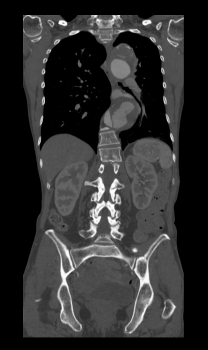
\includegraphics[width=0.4\textwidth]{contraste_osso}} \qquad
  \subfloat[Lung]{\label{fig:contrast_isq}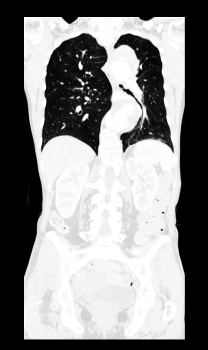
\includegraphics[width=0.4\textwidth]{contraste_pulmao}}
  \caption{Different types of brightness and contrast}
  \label{fig:two_window_level}
\end{figure}

\section{Pseudo color}

Another feature to improve the visualization of the images is the pseudo color. This replaces gray levels by color, or by inverted gray levels. In the latter case, previously clear regions of the image become darker and vice versa.

To change the view using a pseudo color, position the mouse cursor over the image and \textbf{right-click} to open a context menu on it. When the menu opens, select the entry \textbf{Pseudo color}, and then click on the desired pseudo color option, as shown in Figure~\ref{fig:pseudo_color}.

\begin{figure}[p]
\centering
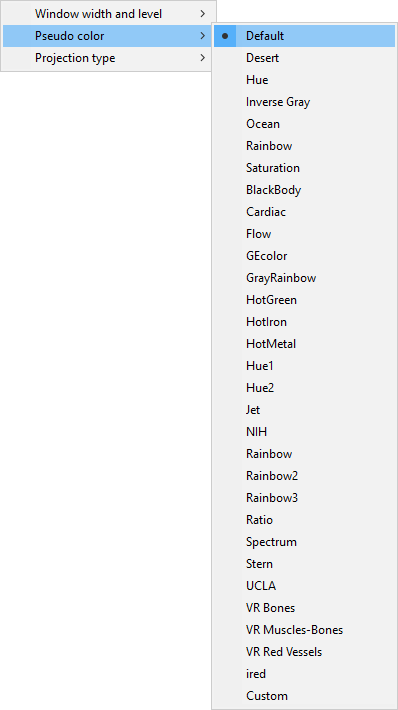
\includegraphics[scale=0.40]{pseudo_menu_en.png}
\caption{Pseudo Color}
\label{fig:pseudo_color}
\end{figure}

Figures~\ref{fig:image_default}a-g demonstrate the various pseudo color options available.

\begin{figure}[h]
  \centering
  \subfloat[Default]{\label{fig:image_default}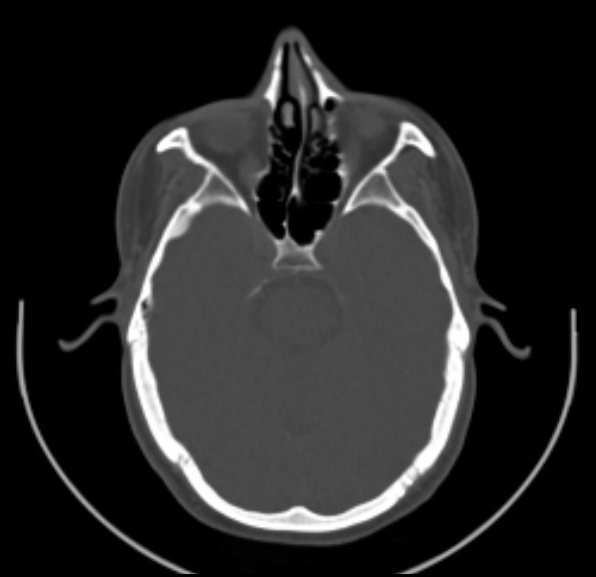
\includegraphics[width=0.25\textwidth]{pseudo_default.jpg}} \qquad
  \subfloat[Inverted Gray Image]{\label{fig:image_inverted}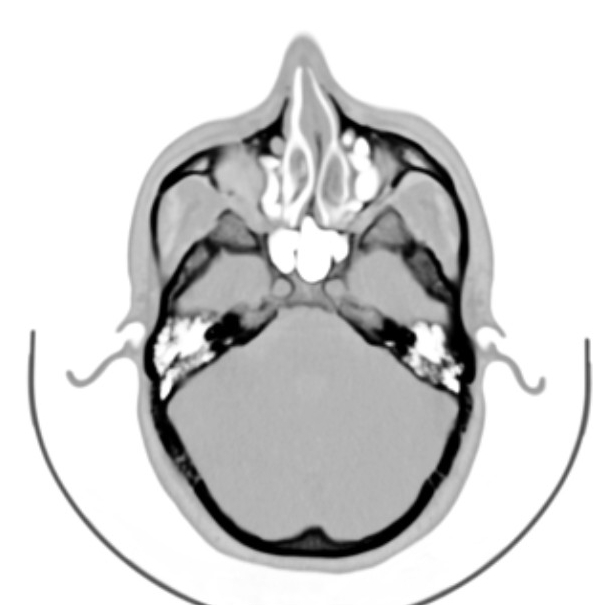
\includegraphics[width=0.25\textwidth]{pseudo_inverse.jpg}} \qquad
  \subfloat[Rainbow]{\label{fig:image_arc}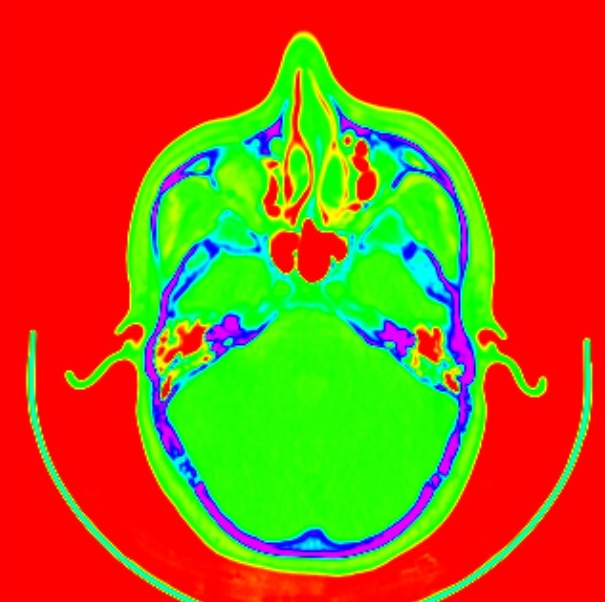
\includegraphics[width=0.25\textwidth]{pseudo_rainbow.jpg}} \\
  \subfloat[Desert]{\label{fig:image_desert}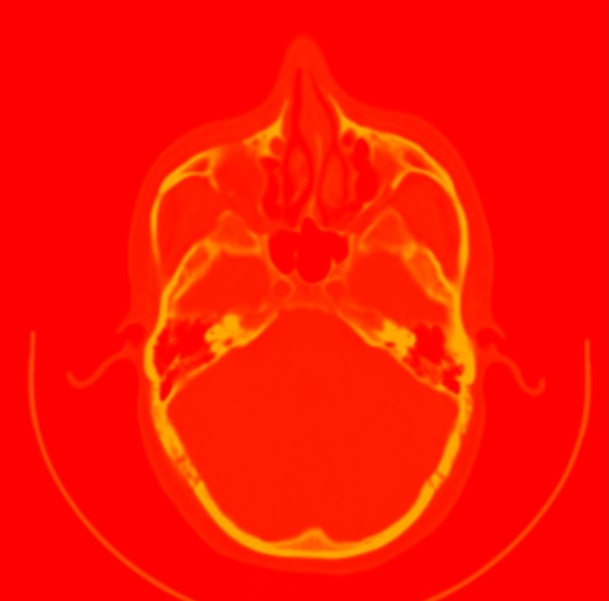
\includegraphics[width=0.25\textwidth]{pseudo_desert.jpg}} \qquad
  \subfloat[Hue]{\label{fig:image_matiz}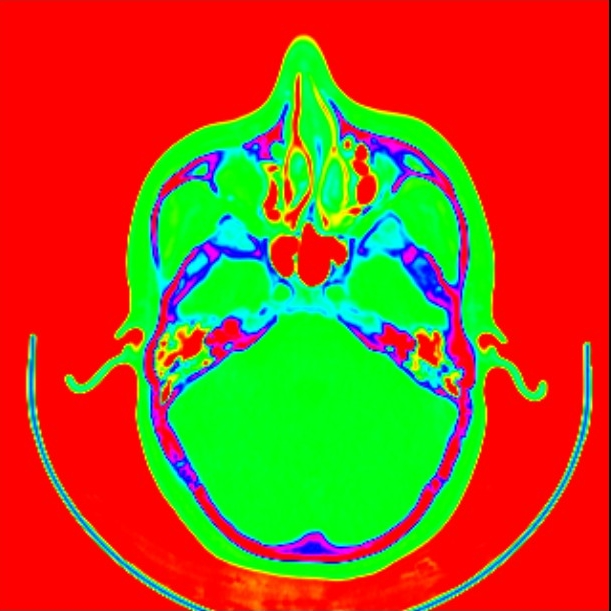
\includegraphics[width=0.25\textwidth]{pseudo_hue.jpg}} \qquad
  \subfloat[Ocean]{\label{fig:image_ocean}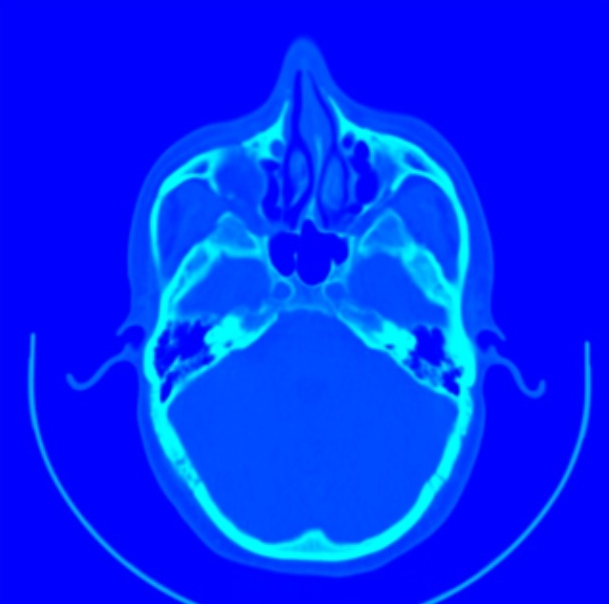
\includegraphics[width=0.25\textwidth]{pseudo_ocean.jpg}}\\
\subfloat[Saturation]{\label{fig:image_saturation}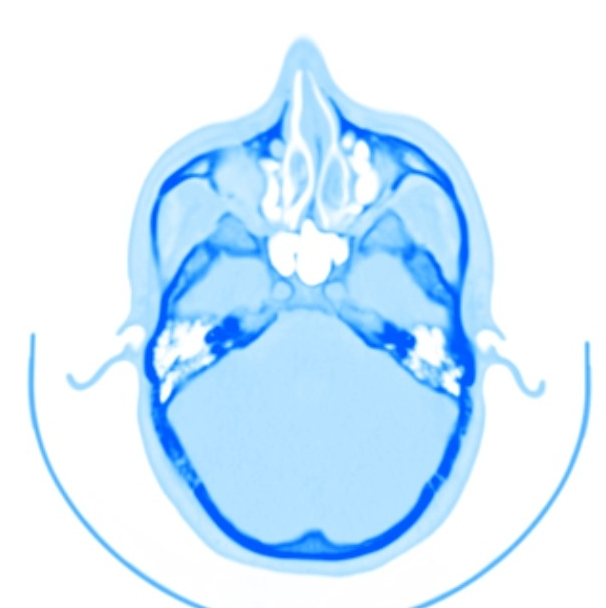
\includegraphics[width=0.25\textwidth]{pseudo_saturation.jpg}}  
  \caption{Some different types of pseudo-color}
  \label{fig:pseudo_color_types}
\end{figure}

\newpage
\section{Projection type}

It is possible to change the projection type of the 2D images, in addition to the normal mode, InVesalius has six types of projections that can be accessed as follows: Place the mouse over the image and \textbf{rigth-click} to open a context menu on it. When the menu opens, select the projection type option, and then click on the desired projection option, as shown in the Figure~\ref{fig:menu_proj}.

\begin{figure}[!h]
\centering
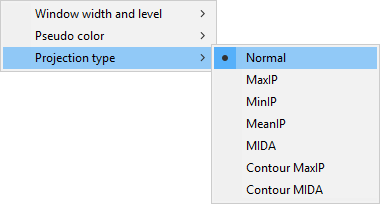
\includegraphics[scale=0.40]{menu_projection_en.png}
\caption{Projection Type menu}
\label{fig:menu_proj}
\end{figure}

\subsection{Normal}

Normal mode is the default view, showing the unmodified image as it was when acquired or customized previously with either brightness and contrast or pseudo color. Normal mode is shown below in Figure~\ref{fig:proj_normal}.

\begin{figure}[!h]
\centering
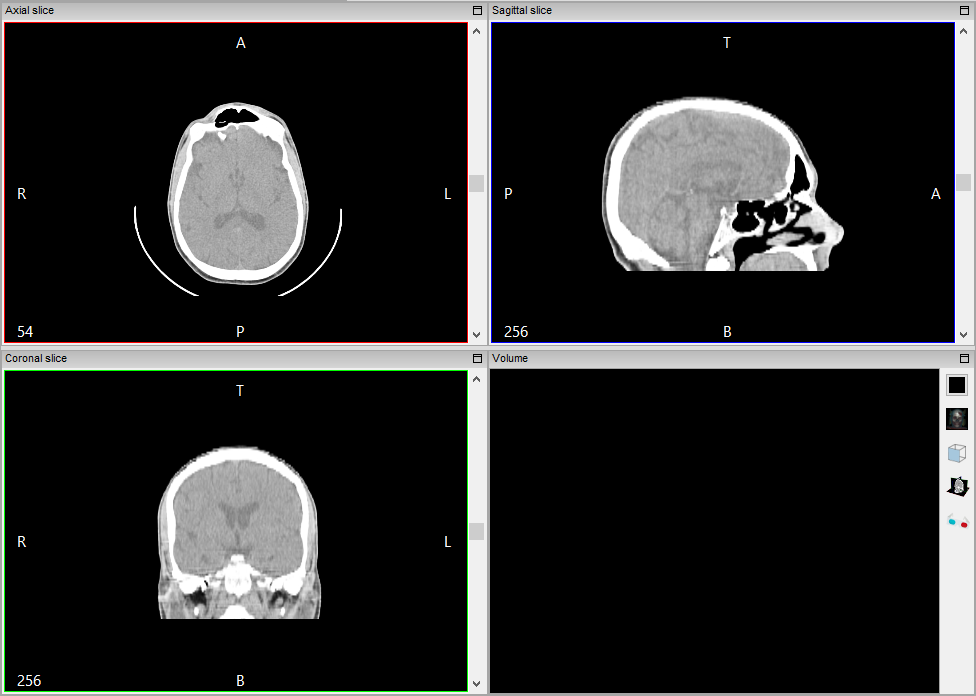
\includegraphics[scale=0.40]{multiplanar_window_en.png}
\caption{Normal projection}
\label{fig:proj_normal}
\end{figure}

\subsection{MaxIP}
\label{sec:max_ip}

MaxIP is also known as MIP (\textit{Maximum Intensity Projection}). MaxIP selects only voxels that have maximum intensity among those visited as shown in Figure~\ref{fig:proj_maxip}. According to the amount of, or "depth" of MaxIP, each voxel is visited in order of overlap, for example, to select MaxIP of the pixel $(0, 0)$ consisting of 3 slices it is necessary to visit pixel $(0, 0)$ of slices $(1, 2, 3)$ and select the highest value.

\begin{figure}[!h]
\centering
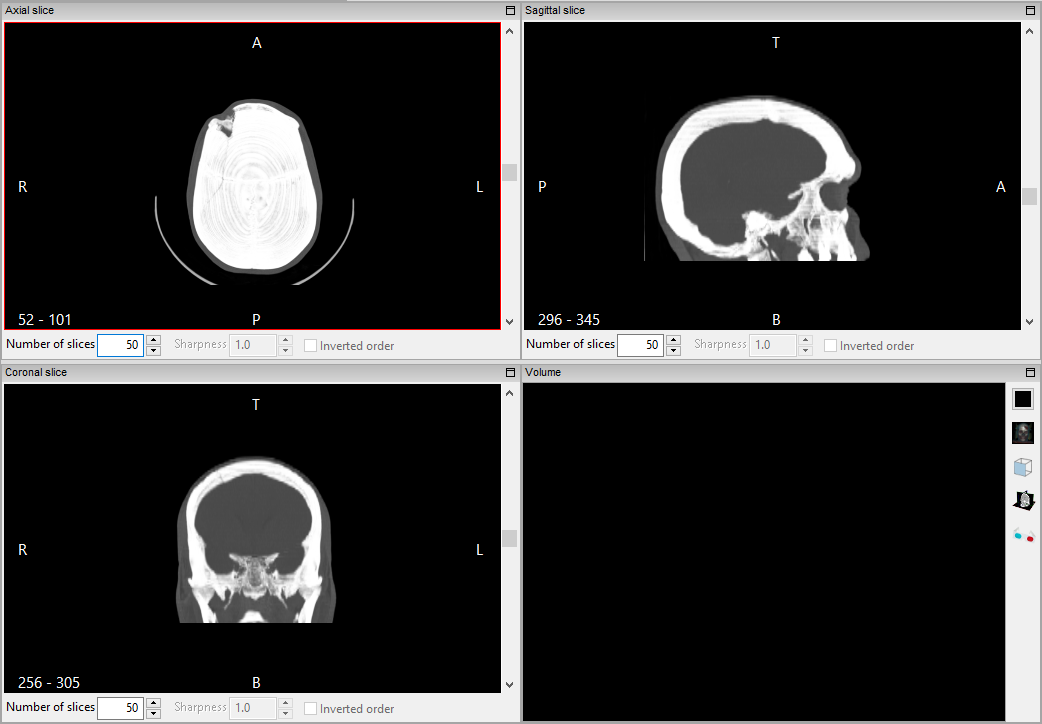
\includegraphics[scale=0.40]{multiplanar_window_maxip_en.png}
\caption{MaxIP projection}
\label{fig:proj_maxip}
\end{figure}

As shown in Figure~\ref{fig:proj_maxip_qtd}, the number of MaxIP images is set at the bottom of each orientation image.

\begin{figure}[!h]
\centering
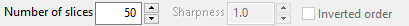
\includegraphics[scale=0.80]{multiplanar_window_maxip_number_en.png}
\caption{Selection the amount of images that composes the MaxIP or MIP}
\label{fig:proj_maxip_qtd}
\end{figure}

\subsection{MinIP}

Unlike MaxIP, MinIP (\textit{Minimum Intensity Projection}) selects only the voxels that have minimal intensity among those visited, as shown in Figure~\ref{fig:proj_minIP}. The image number selection comprising the projection is made at the bottom of each orientation image as shown in Figure~\ref{fig:proj_maxip_qtd}.

\begin{figure}[!h]
\centering
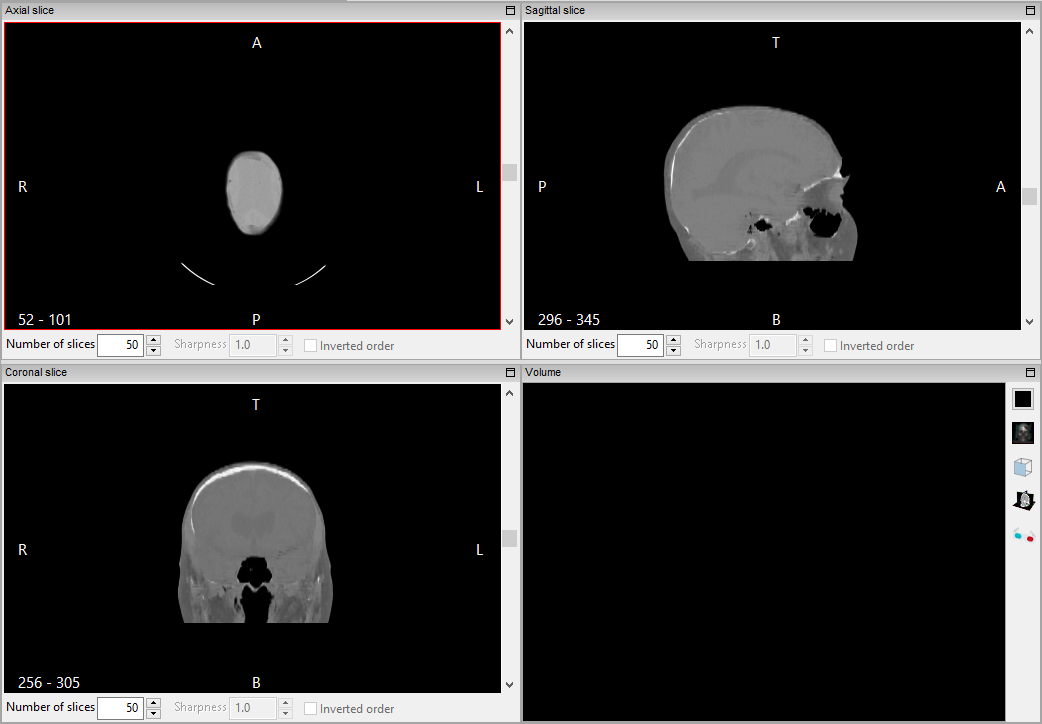
\includegraphics[scale=0.40]{multiplanar_window_minip_en.png}
\caption{MinIP projection}
\label{fig:proj_minIP}
\end{figure}

\subsection{MeanIP}
The MeanIP (\textit{Mean Intensity Projection}) technique which is shown in the Figure~\ref{fig:proj_meanIP} composes the projection by averaging voxels visited in the same way as the MaxIP and MinIP methods. It is also possible to define how many images will compose the projection at the bottom of the image of each orientation as shown in Figure~\ref{fig:proj_maxip_qtd}.

\begin{figure}[!h]
\centering
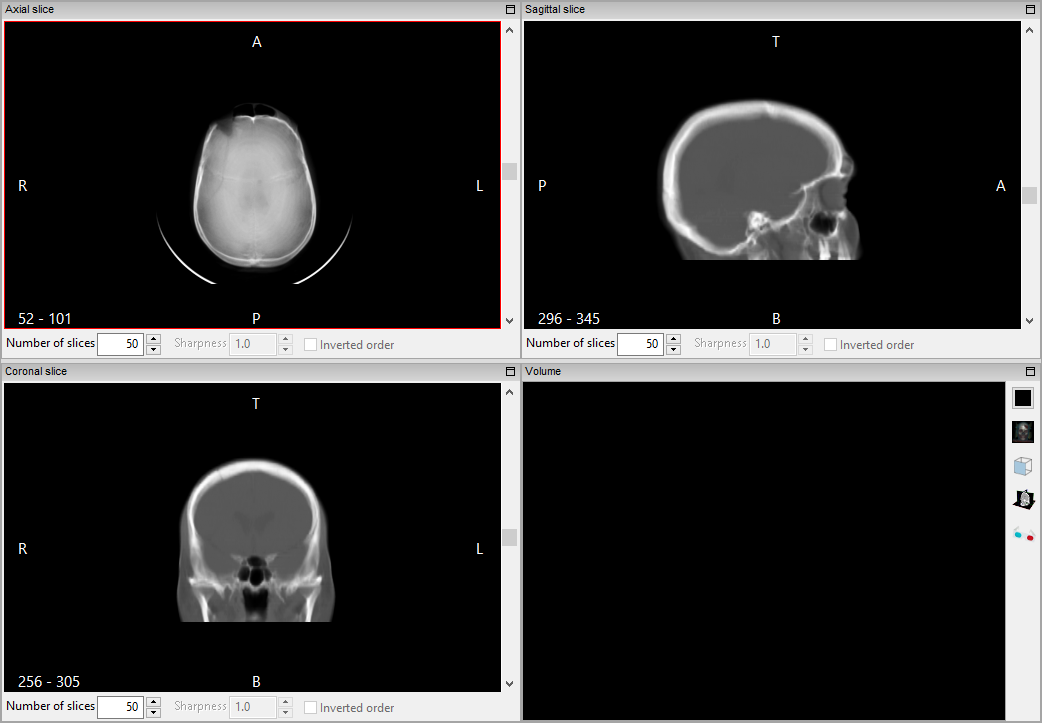
\includegraphics[scale=0.40]{multiplanar_window_mean_en.png}
\caption{MeanIP projection}
\label{fig:proj_meanIP}
\end{figure}

\subsection{MIDA}
\label{sub:mida}
The MIDA (\textit{Maximum Intensity Difference Accumulation}) technique projects an image taking into account only voxels that have local maximum values. From each pixel a ray is simulated towards the volume, with each voxel being intercepted by each ray reaching the end of the volume. Each of the voxels visited has its accumulated value, but are taken into account only if the value is greater than previously visited values. Like MaxIP, one can select how many images are used to accumulate the values. Figure~\ref{fig:proj_MIDA} shows an example of MIDA projection.

\begin{figure}[!h]
\centering
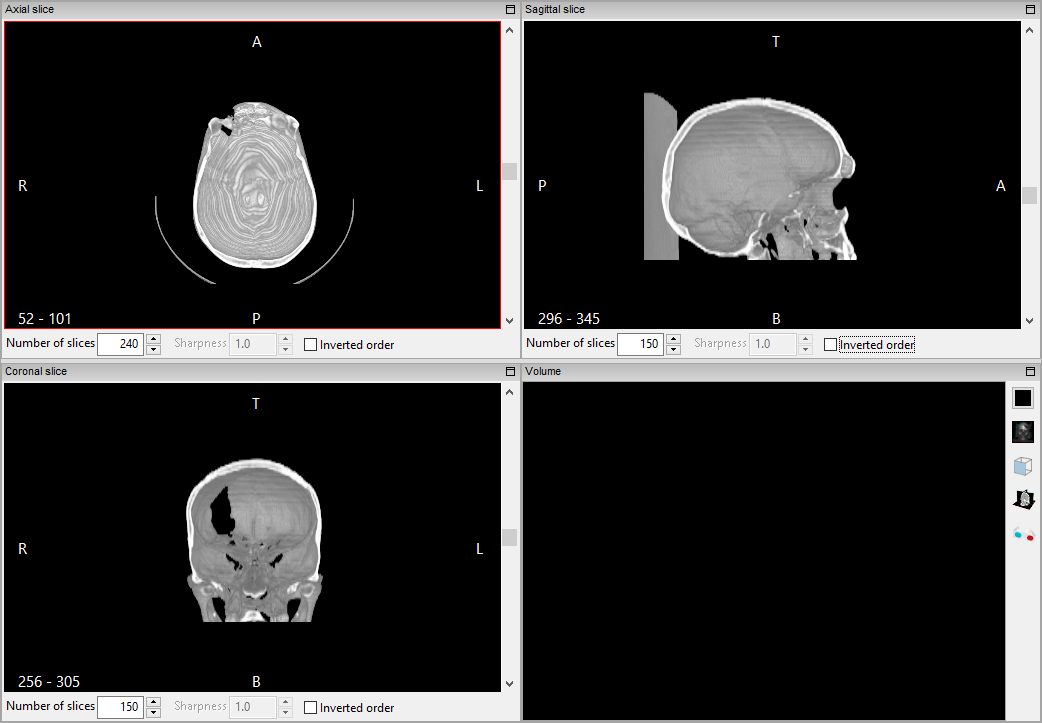
\includegraphics[scale=0.40]{multiplanar_window_mida_en.png}
\caption{MIDA projection}
\label{fig:proj_MIDA}
\end{figure}

As Figure~\ref{fig:proj_MIDA_inv} shows, it is possible to invert the order that the voxels are visited by selecting the \textbf{Inverted order} option in the lower corner of the screen.

\begin{figure}[!h]
\centering
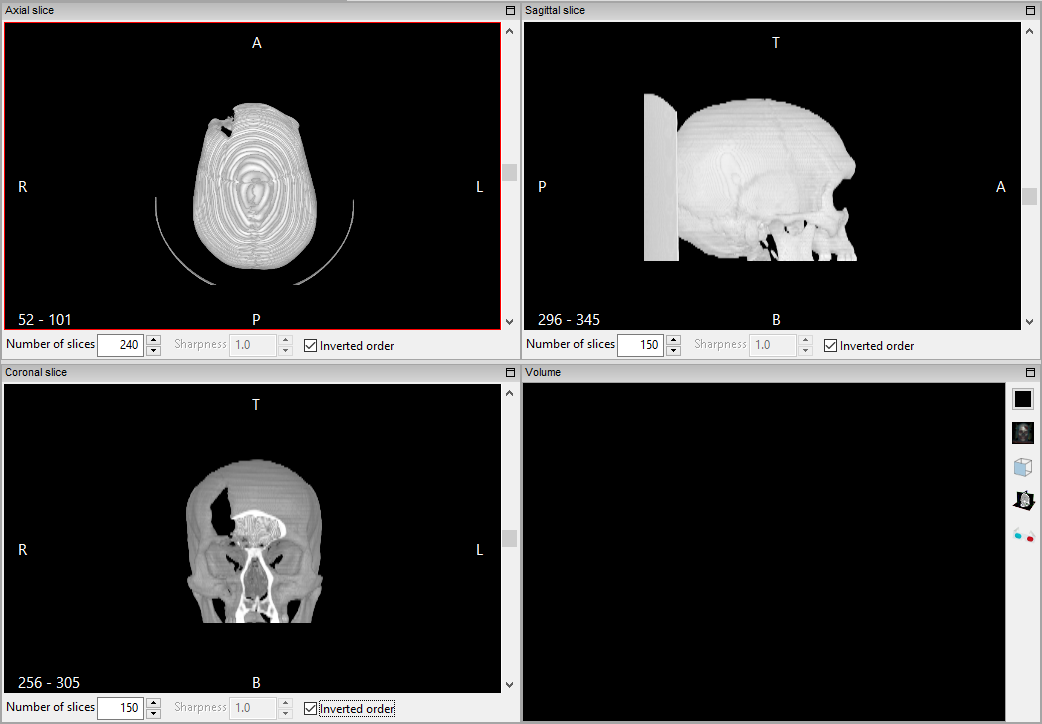
\includegraphics[scale=0.40]{multiplanar_window_mida_inverted_en.png}
\caption{Inverted order MIDA projection}
\label{fig:proj_MIDA_inv}
\end{figure}

\subsection{Contour MaxIP}

The Contour MaxIP function consists of visualizing contours present in the projection generated with MaxIP technique(\ref{sec:max_ip}). An example is presented in Figure~\ref{fig:proj_contorno_maxip}.

\begin{figure}[!h]
\centering
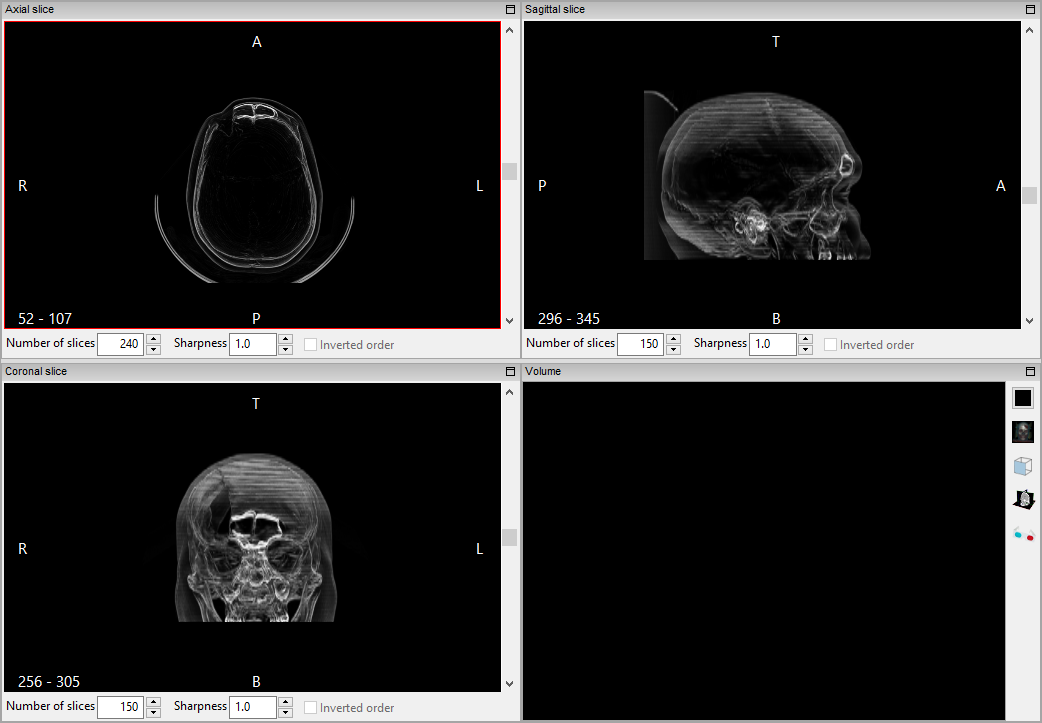
\includegraphics[scale=0.40]{multiplanar_window_contour_maxip_en.png}
\caption{Contour MaxIP projection}
\label{fig:proj_contorno_maxip}
\end{figure}

\subsection{Contour MIDA}

The Contour MIDA function consists of visualizing contours present in the projection generated with the MIDA technique(\ref{sub:mida}). Like MIDA, you can reverse the order that the volume is visited, as shown in Figure~\ref{fig:proj_contorno_mida}.

\begin{figure}[!h]
\centering
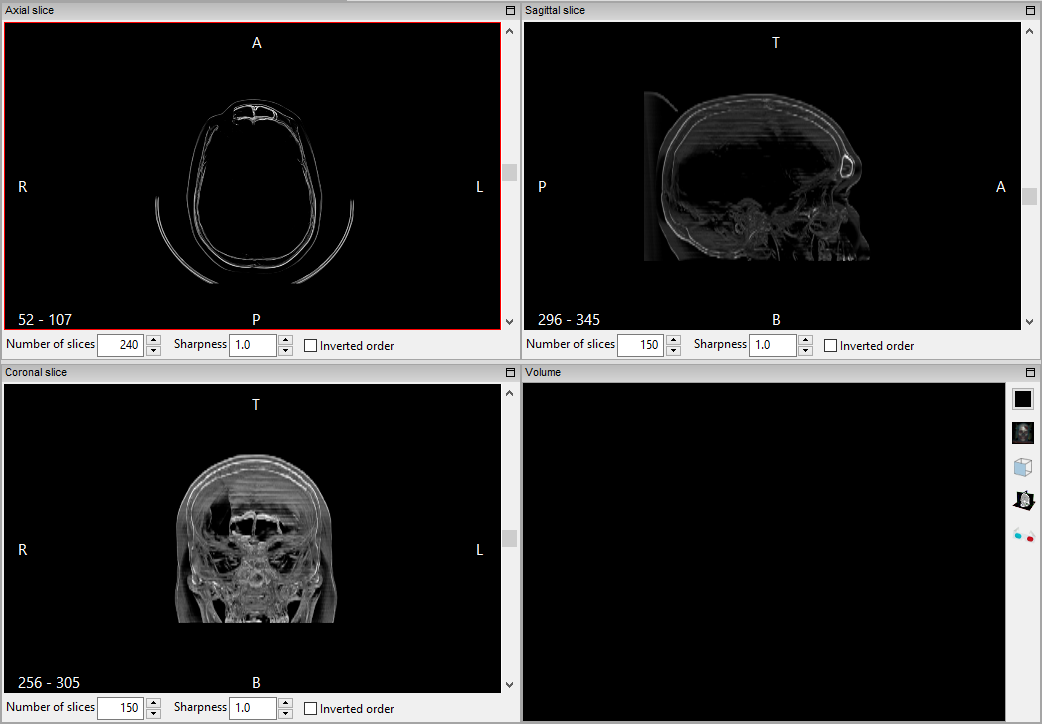
\includegraphics[scale=0.40]{multiplanar_window_contour_mida_en.png}
\caption{Contour MIDA projection}
\label{fig:proj_contorno_mida}
\end{figure}
